%%===========================================================%%
%%                                                           %%
%%                   SYSTEMATIC ERRORS                       %%
%%                                                           %%
%%===========================================================%%


\chapter{Systematic errors}\label{chap:systematicErrors}
\section{TPC track reconstruction efficiency}\label{sec:tpcSystematics}
\subsection{Embedding (pile-up) effect}\label{subsec:TpcEffSystPileUp}
One major difference between simulation and real data is the presence of pile-up
events. The average number of pile-up tracks in
a triggering event is proportional to the BBC coincidence rate. It is expected that
the difference between simulation and real data drops at lower BBC rates, and the
effects of pile-up tracks could be much reduced by fitting the tracking efficiency as a
function of BBC rate and using the extrapolated value at zero luminosity to compare
with simulation.\newline

%---------------------------
\begin{wrapfigure}{r}{0.45\textwidth}\vspace*{-9pt}
	\centering
	\includegraphics[width=0.45\textwidth, page=5]{graphics/systematicsEfficiency/bbc_and/Out.pdf}
	\caption[Number of events in embedded MC as a function of BBC\_AND rate.]
	{Number of events in embedded MC as a function of BBC\_AND rate. The black and red lines represent the events with \mbox{$<\text{BBC\_AND}>=700$~kHz} and \mbox{$<\text{BBC\_AND}>=1400$~kHz},  respectively.}
	\label{fig:events_bbc_and}%\vspace*{-29pt}
\end{wrapfigure}
%---------------------------
\noindent The embedded MC was divided into two samples due to mean BBC\_AND rate: \mbox{$<\text{BBC\_AND}>=700$~kHz} and \mbox{$<\text{BBC\_AND}>=1400$~kHz}. Next, the track reconstruction efficiency was calculated for those two samples and no-pile-up MC corresponding to them. The difference between TPC track reconstruction efficiences for pile-up and no-pile-up MCs was calculated as:
\begin{equation}
	\Delta\epsilon_{ TPC}^{1400/700\text{ kHz}} = \frac{N_{reco}^{no-pile-up}-N_{reco}^{pile-up}}{N_{gen}}\\
	\label{eq:tpcSyst}
\end{equation}
where:\\
$N_{gen}$-number of MC tracks,\\
$N_{reco}^{no-pile-up}$ - number of reconstructed tracks, matched with MC tracks in no-pile-up MC,\\
$N_{reco}^{pile-up}$ - number of reconstructed tracks, matched with MC tracks in pile-up MC.

The difference between high and low pile-up runs is given by:
\begin{equation}
\Delta\epsilon_{ TPC} =\Delta\epsilon_{ TPC}^{1400\text{ kHz}}-2\cdot\Delta\epsilon_{ TPC}^{700\text{ kHz}}
\label{eq:tpcSystDifference}
\end{equation}
Finally, above difference, shown in  \Cref{fig:systError1Dtpc,fig:systError2Dtpc} for $\pi^\pm$, varies between $2-3\%$ and was taken as systematic uncertainty related to TPC track reconstruction efficiency.
%\vspace{10em}
\begin{figure}[hb]
	\caption[$\pi^\pm$ TPC track reconstruction efficiency as a function of $p_T$ $\left(|\eta|<0.7, |V_z|<80\text{ cm}\right)$ for embedded MC samples with \mbox{$<\text{BBC\_AND}>=700$~kHz} and \mbox{$<\text{BBC\_AND}>=1400$~kHz}]{$\pi^\pm$ TPC track reconstruction efficiency as a function of $p_T$ $\left(|\eta|<0.7, |V_z|<80\text{ cm}\right)$ for embedded MC samples with \mbox{$<\text{BBC\_AND}>=700$~kHz} and \mbox{$<\text{BBC\_AND}>=1400$~kHz}. The efficiences from corresponding no-pile-up MC samples were also shown. Additionally, the differences  from Eq. \ref{eq:tpcSystDifference} were drawn in the bottom of each plot.}
	\label{fig:systError1Dtpc}
	\centering
	\parbox{0.495\textwidth}{
		\centering
		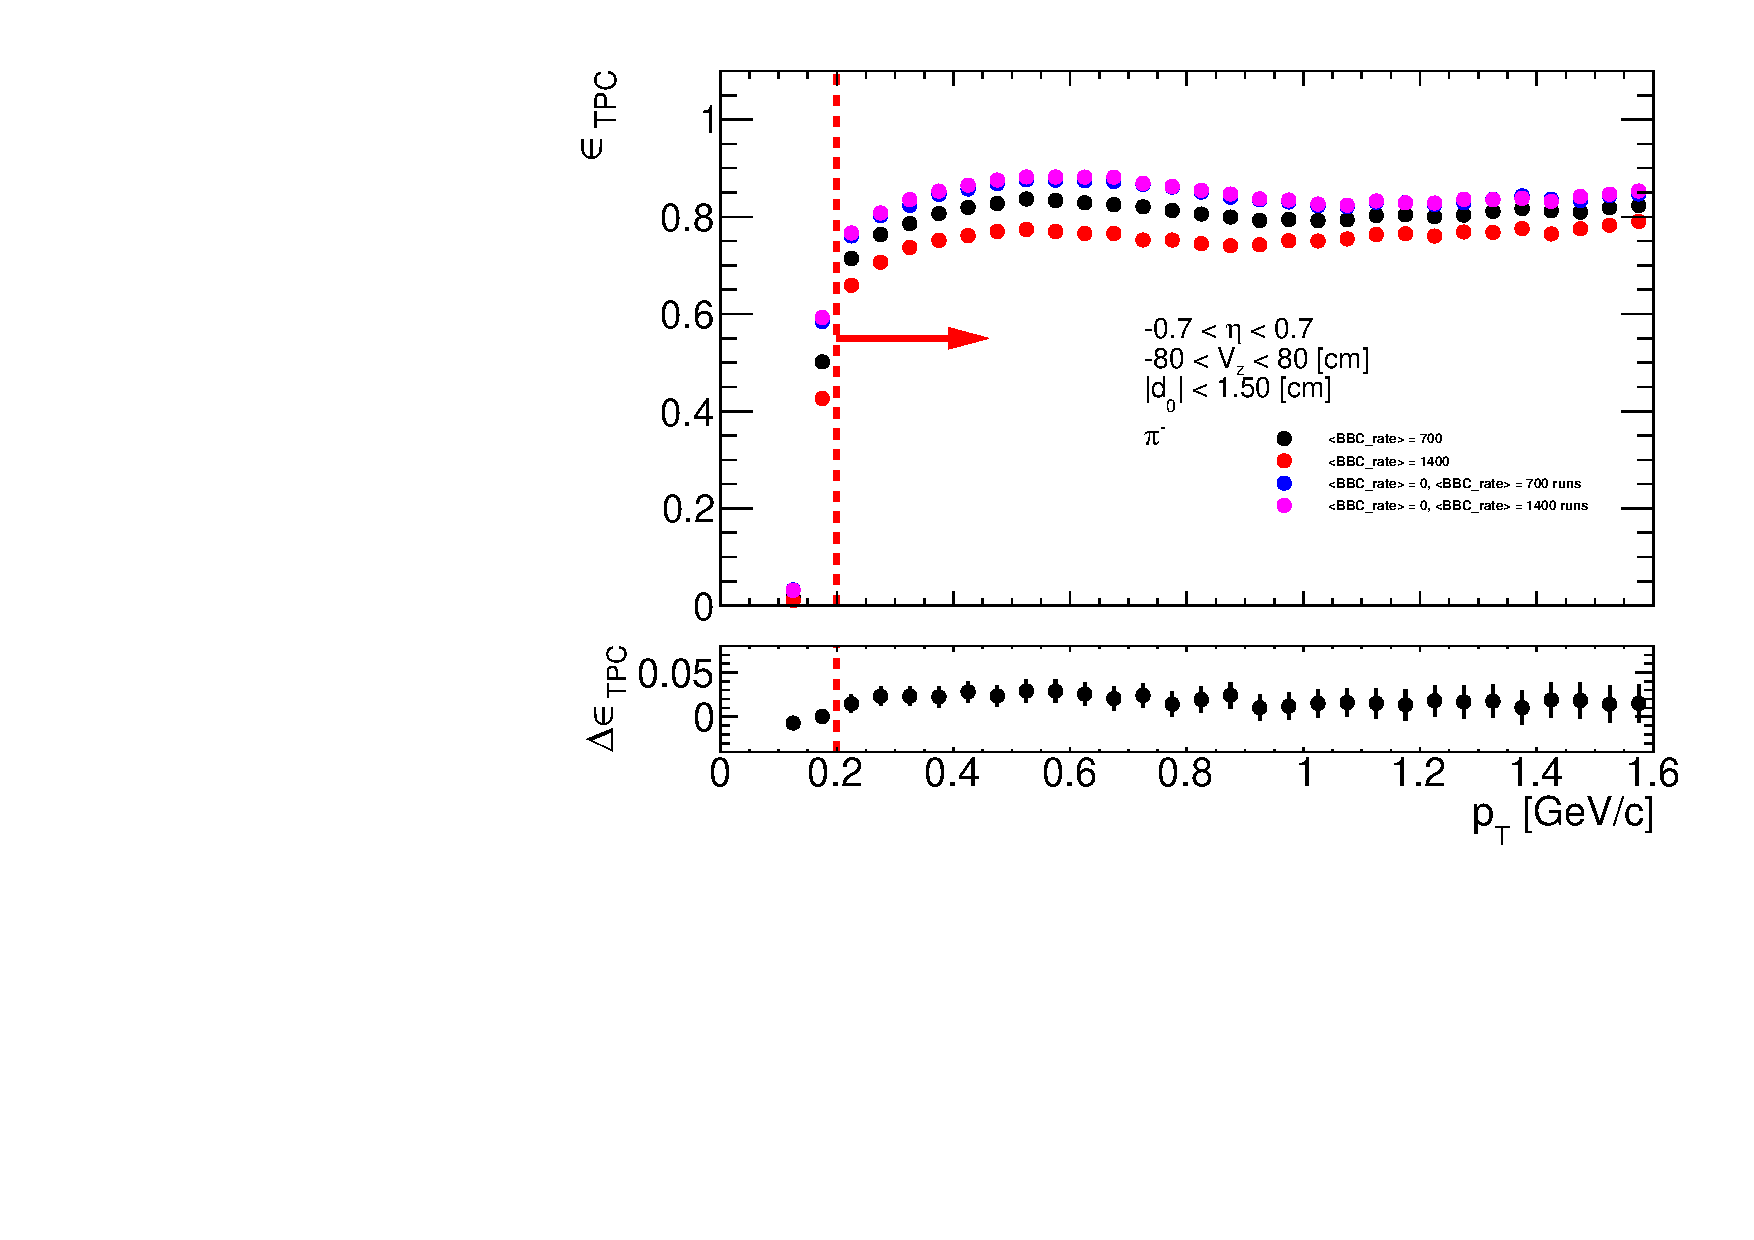
\includegraphics[width=\linewidth,page=1]{graphics/systematicsEfficiency/bbc_and/tpcEffi_d0_1_5_etapt_1.pdf}\\
	}~
	\parbox{0.495\textwidth}{
		\centering
		\includegraphics[width=\linewidth,page=2]{graphics/systematicsEfficiency/bbc_and/tpcEffi_d0_1_5_etapt_1.pdf}\\
	}%
\end{figure}
\begin{figure}[H]
	\caption[The difference $\Delta\epsilon_{ TPC} =\Delta\epsilon_{ TPC}^{1400\text{ kHz}}-2\cdot\Delta\epsilon_{ TPC}^{700\text{ kHz}}$ for $\pi^\pm$ as a function of $p_T$ and $\eta$ $\left(|V_z|<80\text{ cm}\right)$]{The difference $\Delta\epsilon_{ TPC} =\Delta\epsilon_{ TPC}^{1400\text{ kHz}}-2\cdot\Delta\epsilon_{ TPC}^{700\text{ kHz}}$ for $\pi^\pm$ as a function of $p_T$ and $\eta$ $\left(|V_z|<80\text{ cm}\right)$. }
	\label{fig:systError2Dtpc}
	\centering
	\parbox{0.495\textwidth}{
		\centering
		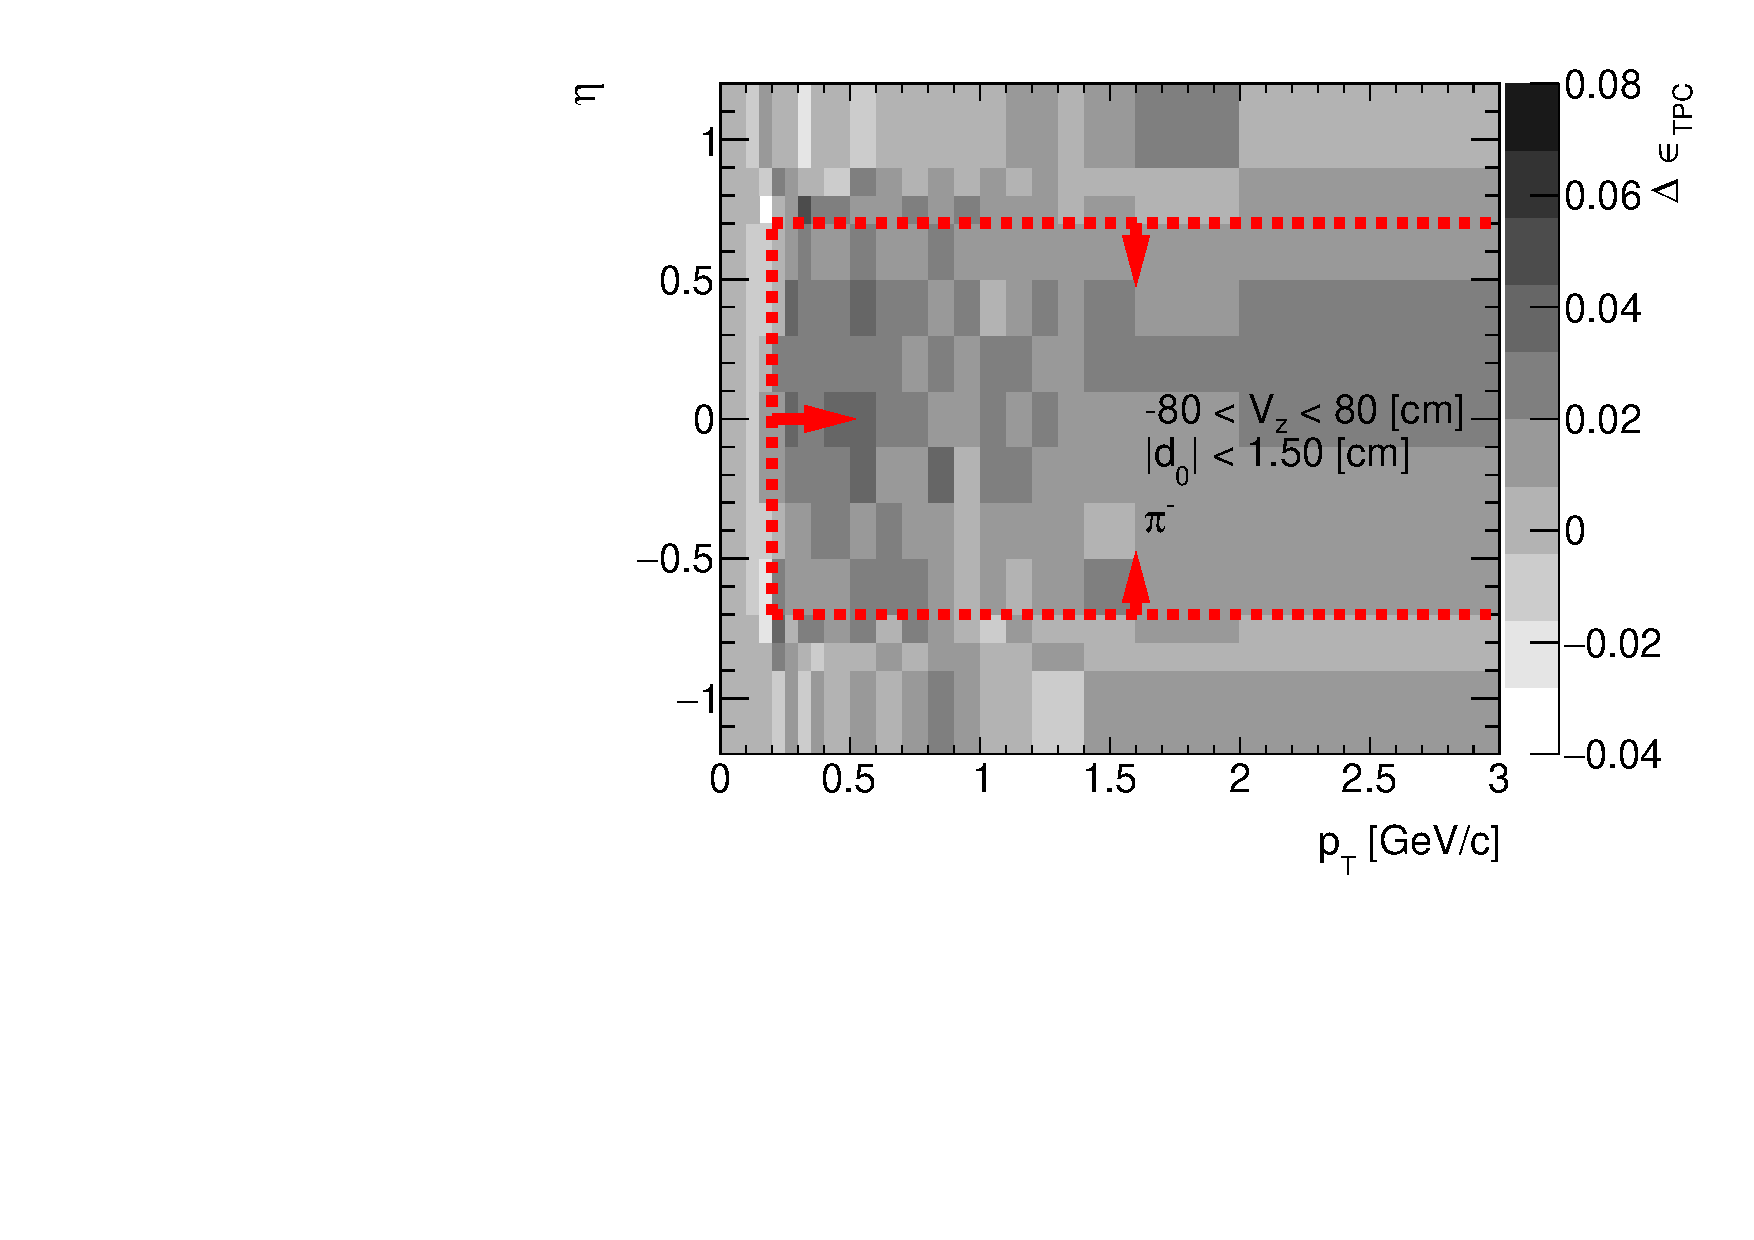
\includegraphics[width=\linewidth,page=1]{graphics/systematicsEfficiency/bbc_and/tpcEffi_d0_1_5_etapt_12D.pdf}\\
	}~
	\parbox{0.495\textwidth}{
		\centering
		\includegraphics[width=\linewidth,page=2]{graphics/systematicsEfficiency/bbc_and/tpcEffi_d0_1_5_etapt_12D.pdf}\\
	}%
\end{figure}

\subsection{Dead material effect on TPC track reconstruction efficiency}\label{sec:deadMaterialSystematics}
The amount of dead material in front of TPC differs up to $20\%$ between data and simulation (see Sec.~\ref{chap:deadMaterial}). First, the~amount of lost particles, $\delta\epsilon_{ TPC}$, due to the interaction with dead material in front of TPC was estimated using  no-pile-up  MC samples. The results for $\pi^-$ in CD are shown in Fig. \ref{fig:dead_materialCD3D}. Then the symmetric systematic uncertainty to the TPC track reconstruction efficiency due to dead material was introduced as $\pm 0.2 \cdot\delta\epsilon_{ TPC}$.
In Fig. \ref{fig:dead_materialCD1D}  the systematic uncertainty is shown for each particle species in CD as a function of $p_T$ $\left(|\eta|<0.7, |V_{z}|<80 \text{ cm}\right)$. 
The results for other particles and SD are shown in Figs. in Appendix \ref{appendix:deadMaterial}.
\begin{figure}[hb]
\caption[The amount of lost $\pi^-$ due to the interaction with dead material in front of TPC as a function of $p_T$, $\eta$ and $z$-vertex in CD]{The amount of lost $\pi^-$ due to the interaction with dead material in front of TPC. Each plot represents the fraction of lost $\pi^-$, $\delta\epsilon_{ TPC}$ ($z$-axis), as a function of true particle pseudorapidity $\eta$ ($y$-axis) and transverse momentum $p_{T}$ ($x$-axis) in single $z$-vertex bin.}\label{fig:dead_materialCD3D}
\centering
\parbox{0.495\textwidth}{
  \centering
  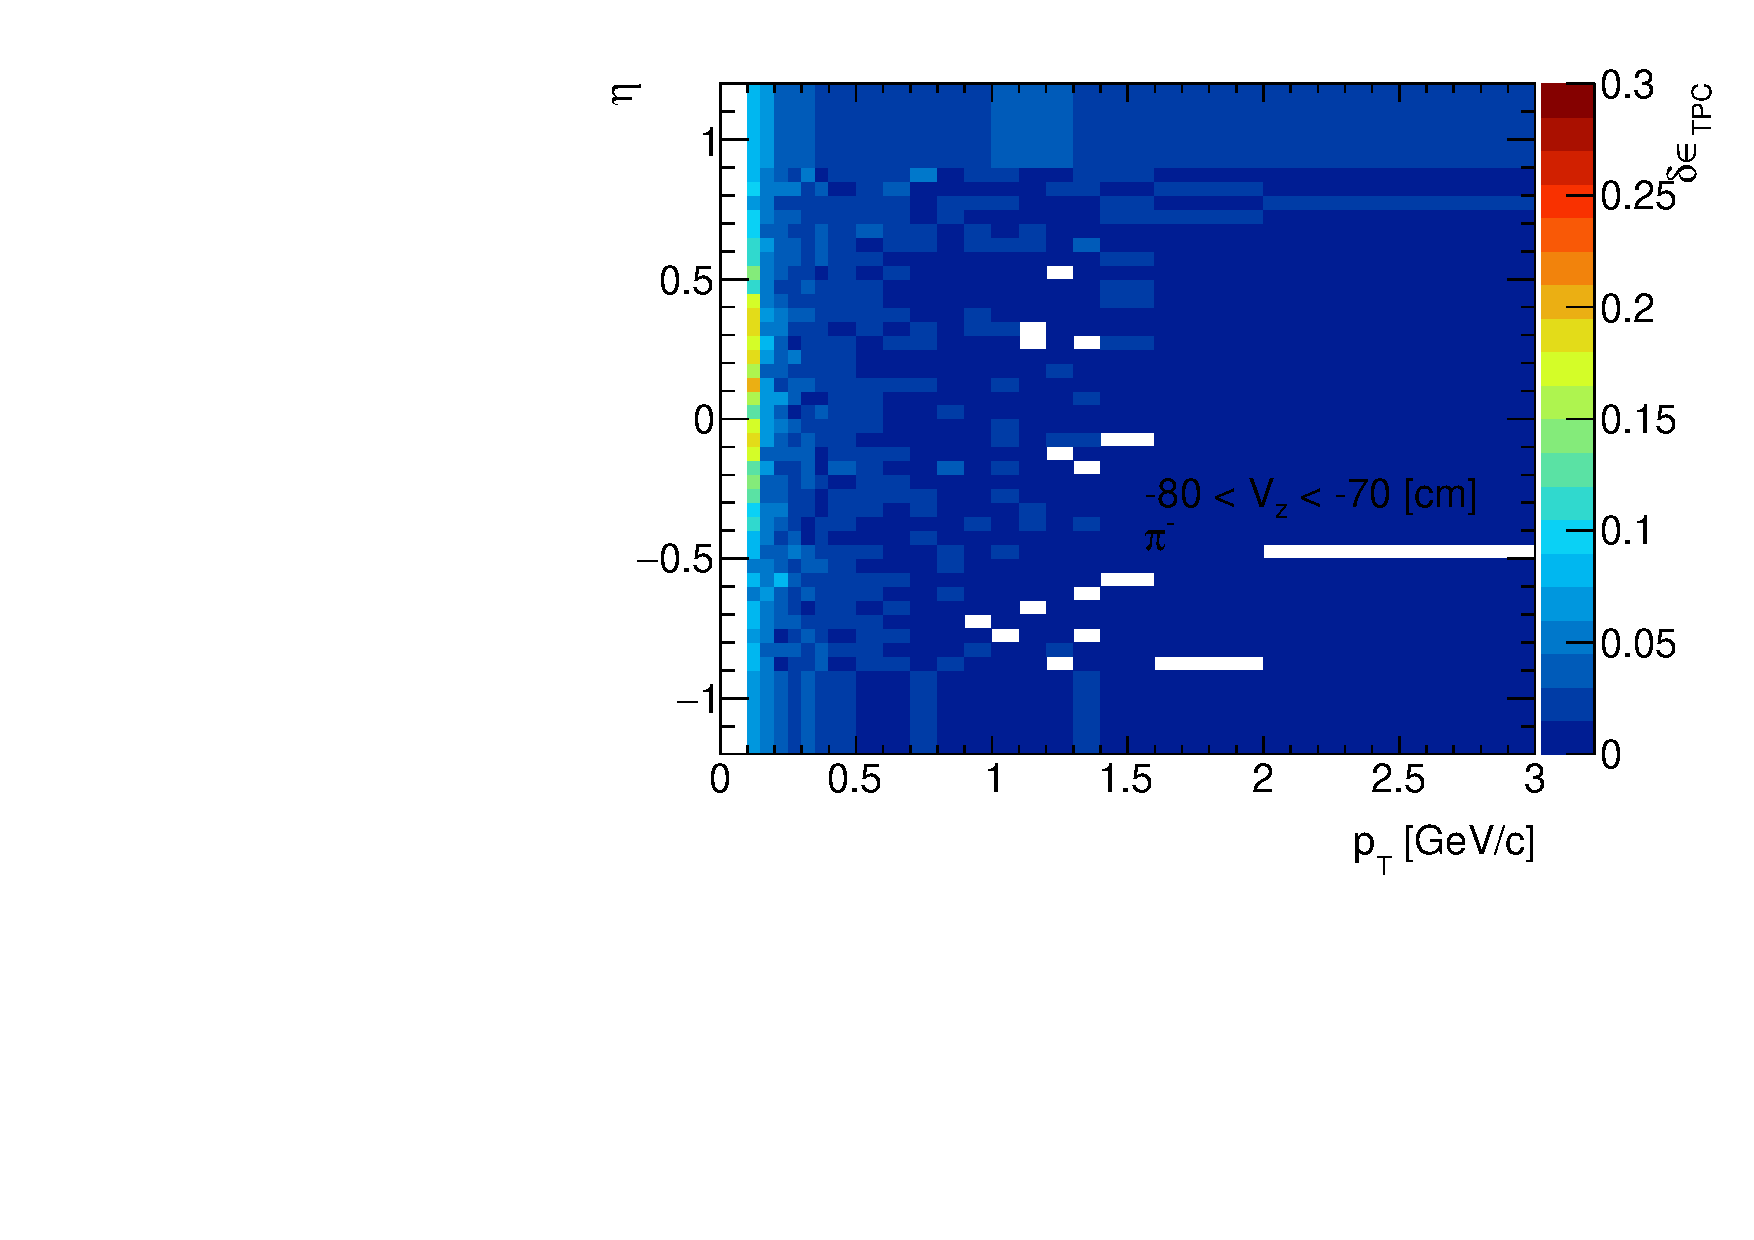
\includegraphics[width=\linewidth,page=1]{graphics/systematicsEfficiency/deadMaterial/secondaries_Unbinned_CD_.pdf}\\
  \includegraphics[width=\linewidth,page=3]{graphics/systematicsEfficiency/deadMaterial/secondaries_Unbinned_CD_.pdf}\\
  \includegraphics[width=\linewidth,page=5]{graphics/systematicsEfficiency/deadMaterial/secondaries_Unbinned_CD_.pdf}\\
  \includegraphics[width=\linewidth,page=7]{graphics/systematicsEfficiency/deadMaterial/secondaries_Unbinned_CD_.pdf}\\
}~
\parbox{0.495\textwidth}{
  \centering
  \includegraphics[width=\linewidth,page=2]{graphics/systematicsEfficiency/deadMaterial/secondaries_Unbinned_CD_.pdf}\\
  \includegraphics[width=\linewidth,page=4]{graphics/systematicsEfficiency/deadMaterial/secondaries_Unbinned_CD_.pdf}\\
  \includegraphics[width=\linewidth,page=6]{graphics/systematicsEfficiency/deadMaterial/secondaries_Unbinned_CD_.pdf}\\
  \includegraphics[width=\linewidth,page=8]{graphics/systematicsEfficiency/deadMaterial/secondaries_Unbinned_CD_.pdf}
}%
\end{figure}
\begin{figure}[hb]\ContinuedFloat
% ~\\[32pt]
\centering
\parbox{0.495\textwidth}{
  \centering
  \includegraphics[width=\linewidth,page=9]{graphics/systematicsEfficiency/deadMaterial/secondaries_Unbinned_CD_.pdf}\\
  \includegraphics[width=\linewidth,page=11]{graphics/systematicsEfficiency/deadMaterial/secondaries_Unbinned_CD_.pdf}\\
  \includegraphics[width=\linewidth,page=13]{graphics/systematicsEfficiency/deadMaterial/secondaries_Unbinned_CD_.pdf}\\
  \includegraphics[width=\linewidth,page=15]{graphics/systematicsEfficiency/deadMaterial/secondaries_Unbinned_CD_.pdf}\\
}~
\parbox{0.495\textwidth}{
  \centering
  \includegraphics[width=\linewidth,page=10]{graphics/systematicsEfficiency/deadMaterial/secondaries_Unbinned_CD_.pdf}\\
  \includegraphics[width=\linewidth,page=12]{graphics/systematicsEfficiency/deadMaterial/secondaries_Unbinned_CD_.pdf}\\
  \includegraphics[width=\linewidth,page=14]{graphics/systematicsEfficiency/deadMaterial/secondaries_Unbinned_CD_.pdf}\\
  \includegraphics[width=\linewidth,page=16]{graphics/systematicsEfficiency/deadMaterial/secondaries_Unbinned_CD_.pdf}
}%
\end{figure}
\begin{figure}[hb]
\caption[The systematic uncertainty to the TPC track reconstruction efficiency due to  amount of dead material in front of TPC using MC samples for CD]{The systematic uncertainty to the TPC track reconstruction efficiency due to  amount of dead material in front of TPC using MC samples for CD. Each plot represents the systematic uncertainty as a~function of true particle $p_T$ $\left(|\eta|<0.7, |V_{z}|<80 \text{ cm}\right)$ for given particle species: $\pi^-$,$\pi^+$, $K^-$, $K^+$, $\bar{p}$ and $p$. It was also calculated for negative and positive particles without identification. }\label{fig:dead_materialCD1D}
\centering
\parbox{0.495\textwidth}{
  \centering
  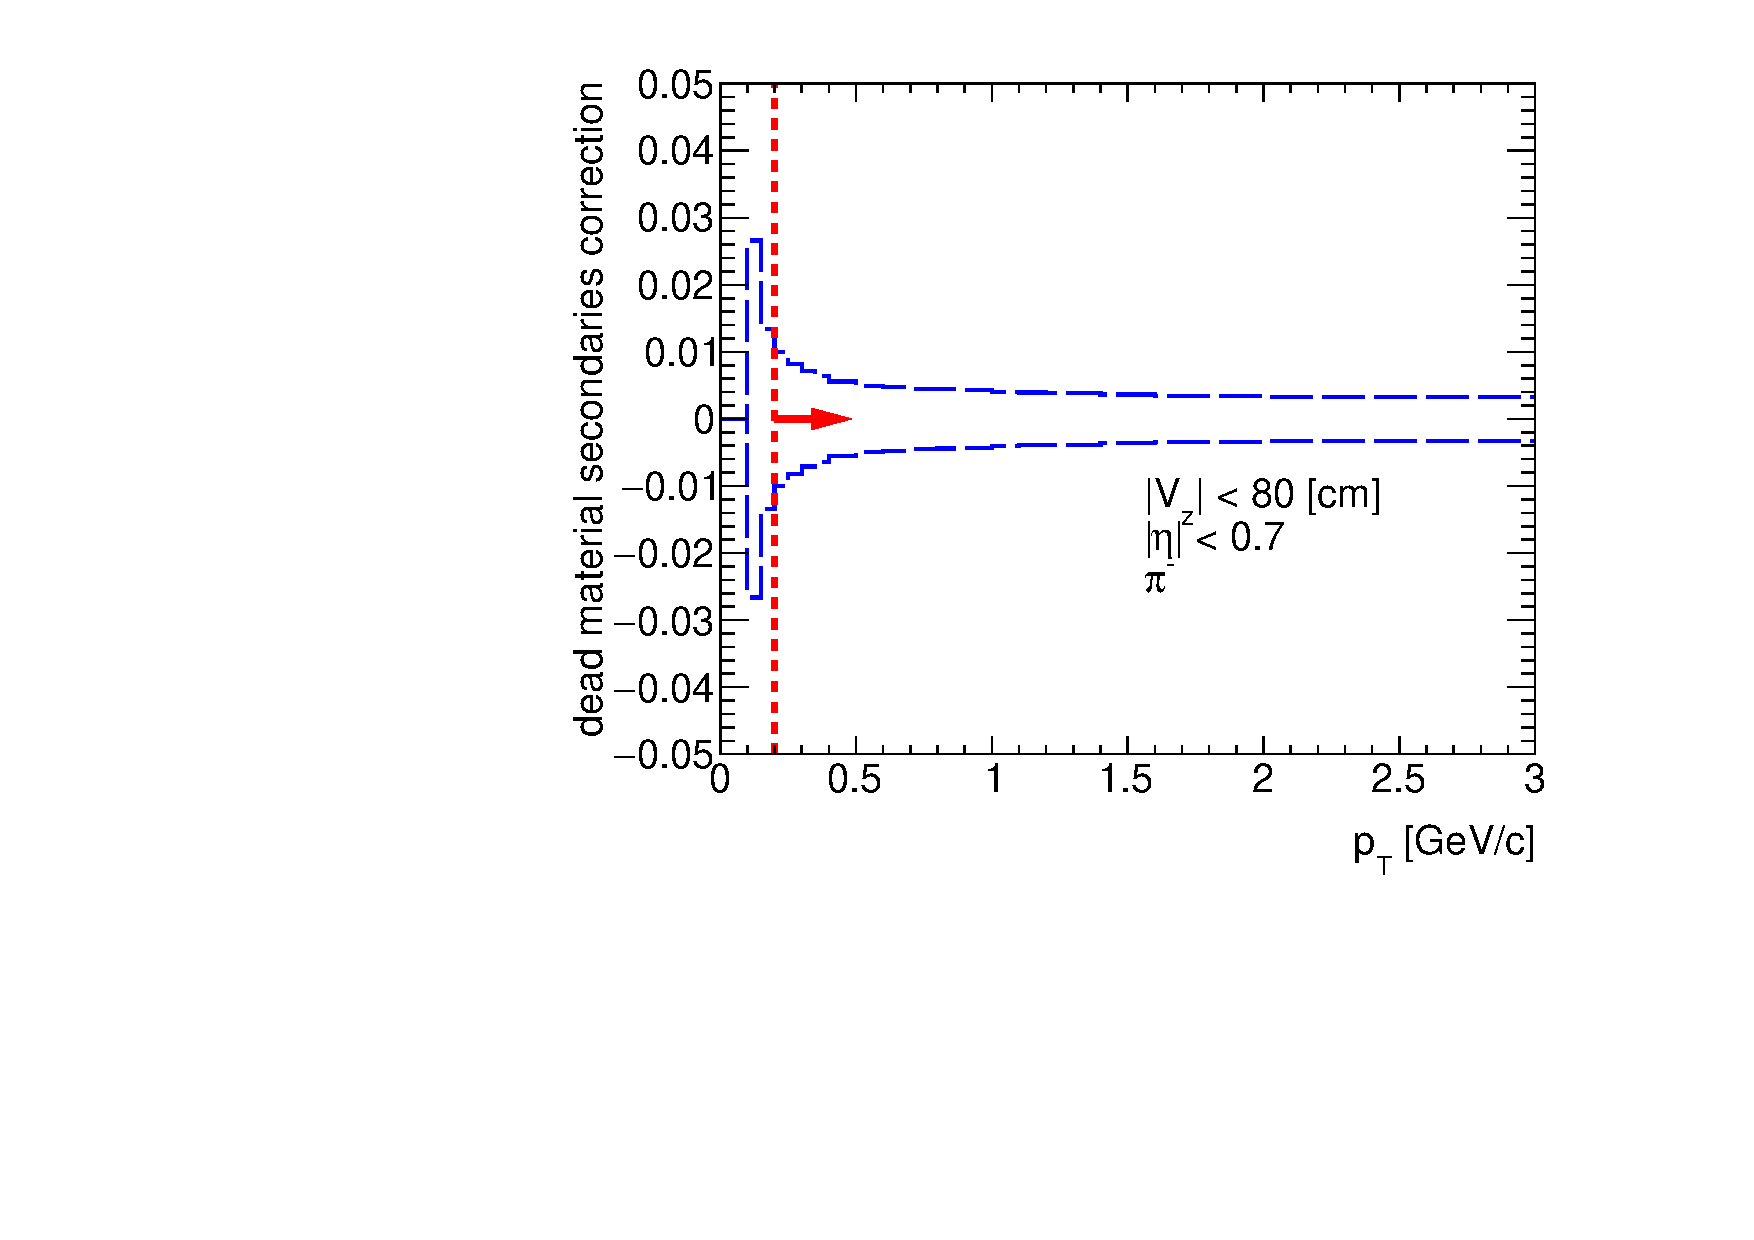
\includegraphics[width=\linewidth,page=1]{graphics/systematicsEfficiency/deadMaterial/secondaries_Unbinned_CD_1D.pdf}\\
  \includegraphics[width=\linewidth,page=2]{graphics/systematicsEfficiency/deadMaterial/secondaries_Unbinned_CD_1D.pdf}\\
  \includegraphics[width=\linewidth,page=3]{graphics/systematicsEfficiency/deadMaterial/secondaries_Unbinned_CD_1D.pdf}\\
  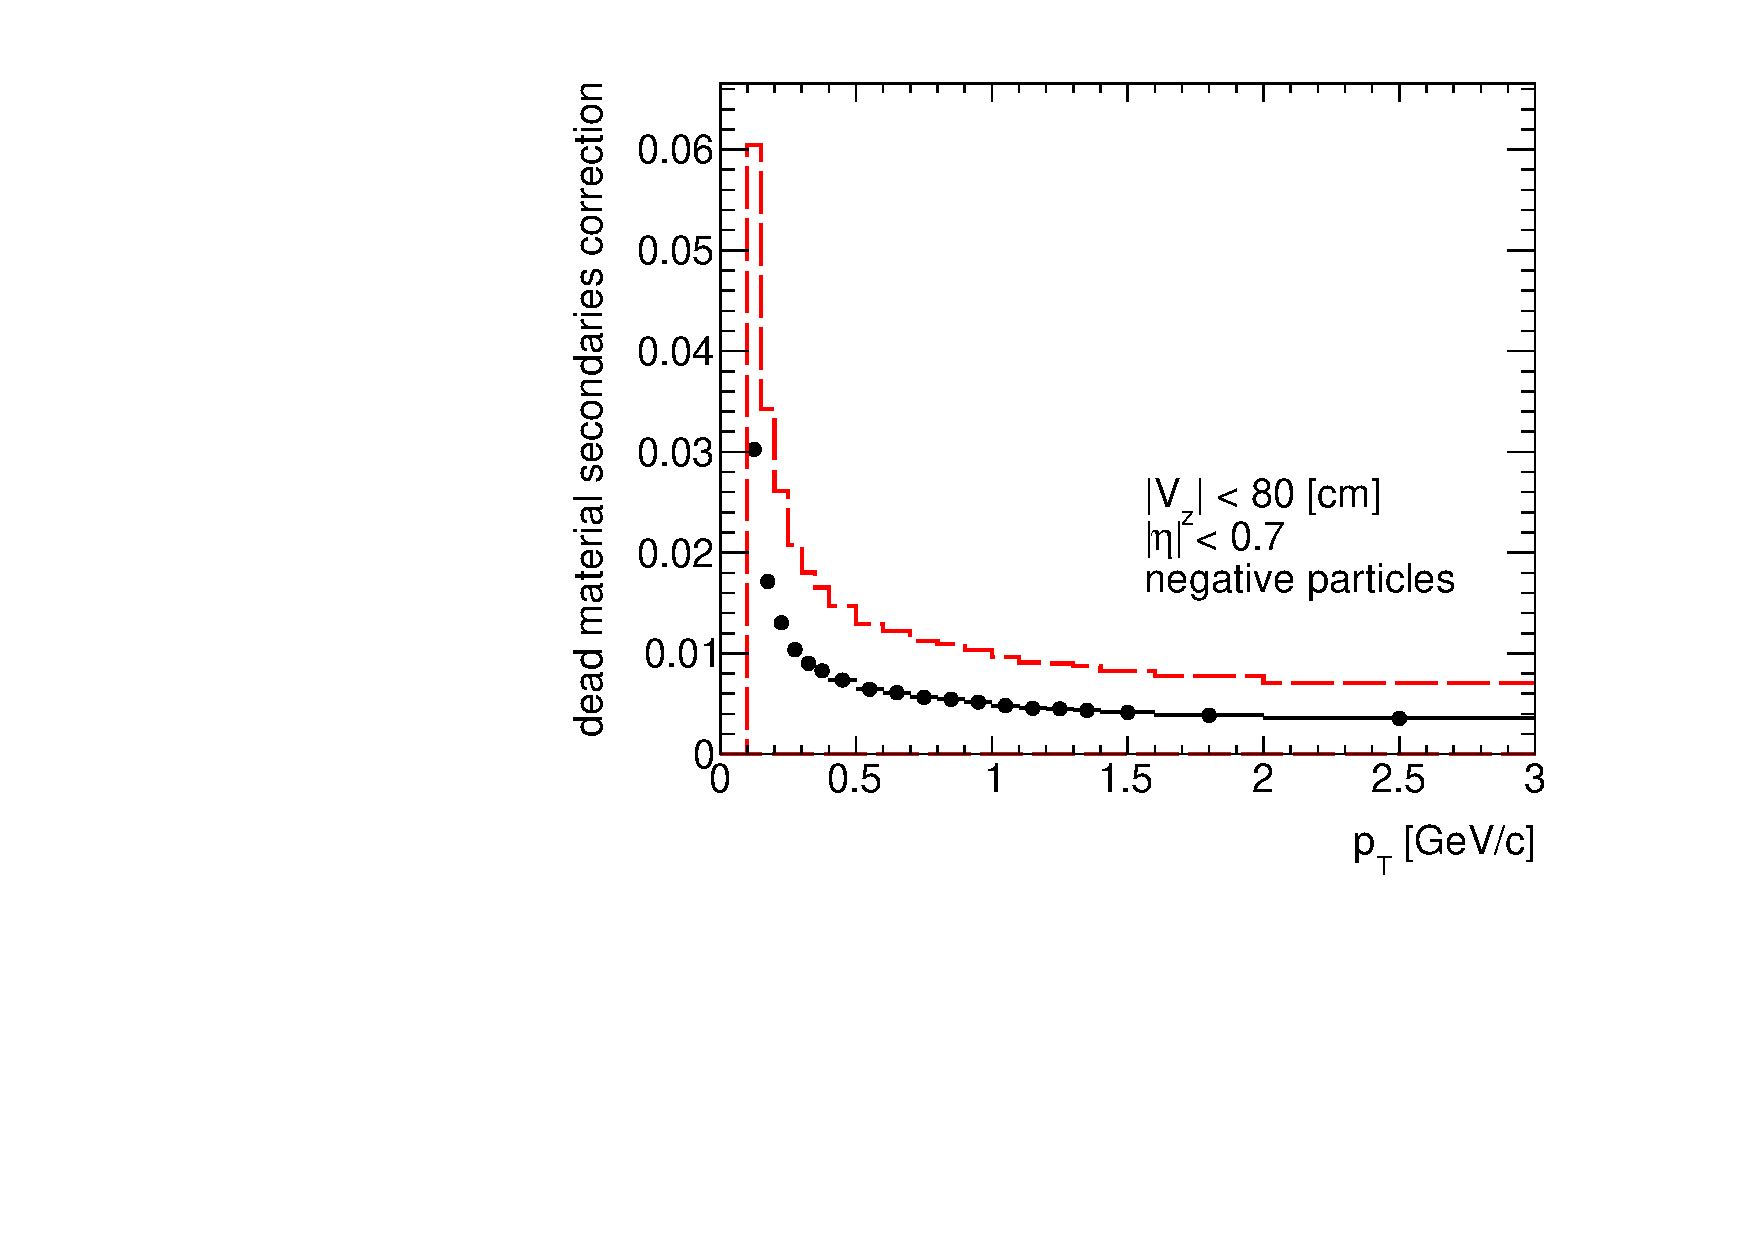
\includegraphics[width=\linewidth,page=1]{graphics/systematicsEfficiency/deadMaterial/secondaries_Unbinned_Charged_CD1D.pdf}\\
}~
\parbox{0.495\textwidth}{
  \centering
  \includegraphics[width=\linewidth,page=4]{graphics/systematicsEfficiency/deadMaterial/secondaries_Unbinned_CD_1D.pdf}\\
  \includegraphics[width=\linewidth,page=5]{graphics/systematicsEfficiency/deadMaterial/secondaries_Unbinned_CD_1D.pdf}\\
  \includegraphics[width=\linewidth,page=6]{graphics/systematicsEfficiency/deadMaterial/secondaries_Unbinned_CD_1D.pdf}\\
  \includegraphics[width=\linewidth,page=2]{graphics/systematicsEfficiency/deadMaterial/secondaries_Unbinned_Charged_CD1D.pdf}
}%
\end{figure}



\section{TOF matching efficiency}\label{sec:tofSystematics}
\subsection{Embedding (pile-up) effect}\label{sec:tofSystematicsPileUpEffect}
The approach to calculate the systematic uncertainty on TOF matching efficiency related to pile-up was quite similar to the one used for TPC track reconstruction efficiency (Sec.~\ref{subsec:TpcEffSystPileUp}). However, the TOF matching efficiency is conditional and depends on TPC track reconstruction efficiency. Since that, the difference between high and low pile-up runs is given by:
\begin{equation}
\Delta\epsilon_{ TOF}^{1400/700\text{ kHz}}=\frac{N_{TPC-TOF}^{no-pile-up}}{N_{TPC}^{no-pile-up}}-\frac{N_{TPC-TOF}^{pile-up}}{N_{TPC}^{pile-up}}
\label{eq:tofSyst}
\end{equation}
where:\\
$N_{TPC-TOF}^{pile-up}$ - number of reconstructed tracks, matched with MC tracks and TOF hit in pile-up MC,\\
$N_{TPC-TOF}^{no-pile-up}$ - number of reconstructed tracks, matched with MC tracks and TOF hit in no-pile-up MC,\\
$N_{TPC}^{pile-up}$ - number of reconstructed tracks, matched with MC tracks in pile-up MC,\\
$N_{TPC}^{no-pile-up}$ - number of reconstructed tracks, matched with MC tracks in no-pile-up MC.

\noindent Next the difference between high and low pile-up events was calculated withe the formula similar to the one given by Eq. \ref{eq:tpcSystDifference} and is shown in \Cref{fig:systError1Dtof,fig:systError2Dtof}. The origin of  $N_{TPC-TOF}$ increase is not known (it may be due to lack of pile-up in TPC or TOF). Since that, it is impossible to correctly calculate the statistical error for $\Delta\epsilon_{ TOF}$. Nevertheless, $\Delta\epsilon_{ TOF}$ is  smaller than $0.5\%$ and can be neglected in comparison with other systematic uncertainties.
\begin{figure}[hb]
	\caption[$\pi^\pm$ TOF matching efficiency as a function of $p_T$ $\left(|\eta|<0.7, |V_z|<80\text{ cm}\right)$ for embedded MC samples with \mbox{$<\text{BBC\_AND}>=700$~kHz} and \mbox{$<\text{BBC\_AND}>=1400$~kHz}]{$\pi^\pm$ TOF matching efficiency as a function of $p_T$ $\left(|\eta|<0.7, |V_z|<80\text{ cm}\right)$ for embedded MC samples with \mbox{$<\text{BBC\_AND}>=700$~kHz} and \mbox{$<\text{BBC\_AND}>=1400$~kHz}. The efficiences from corresponding no-pile-up MC samples were also shown. Additionally, the differences  from Eq. \ref{eq:tpcSystDifference} were drawn in the bottom of each plot.}
	\label{fig:systError1Dtof}
	\centering
	\parbox{0.495\textwidth}{
		\centering
		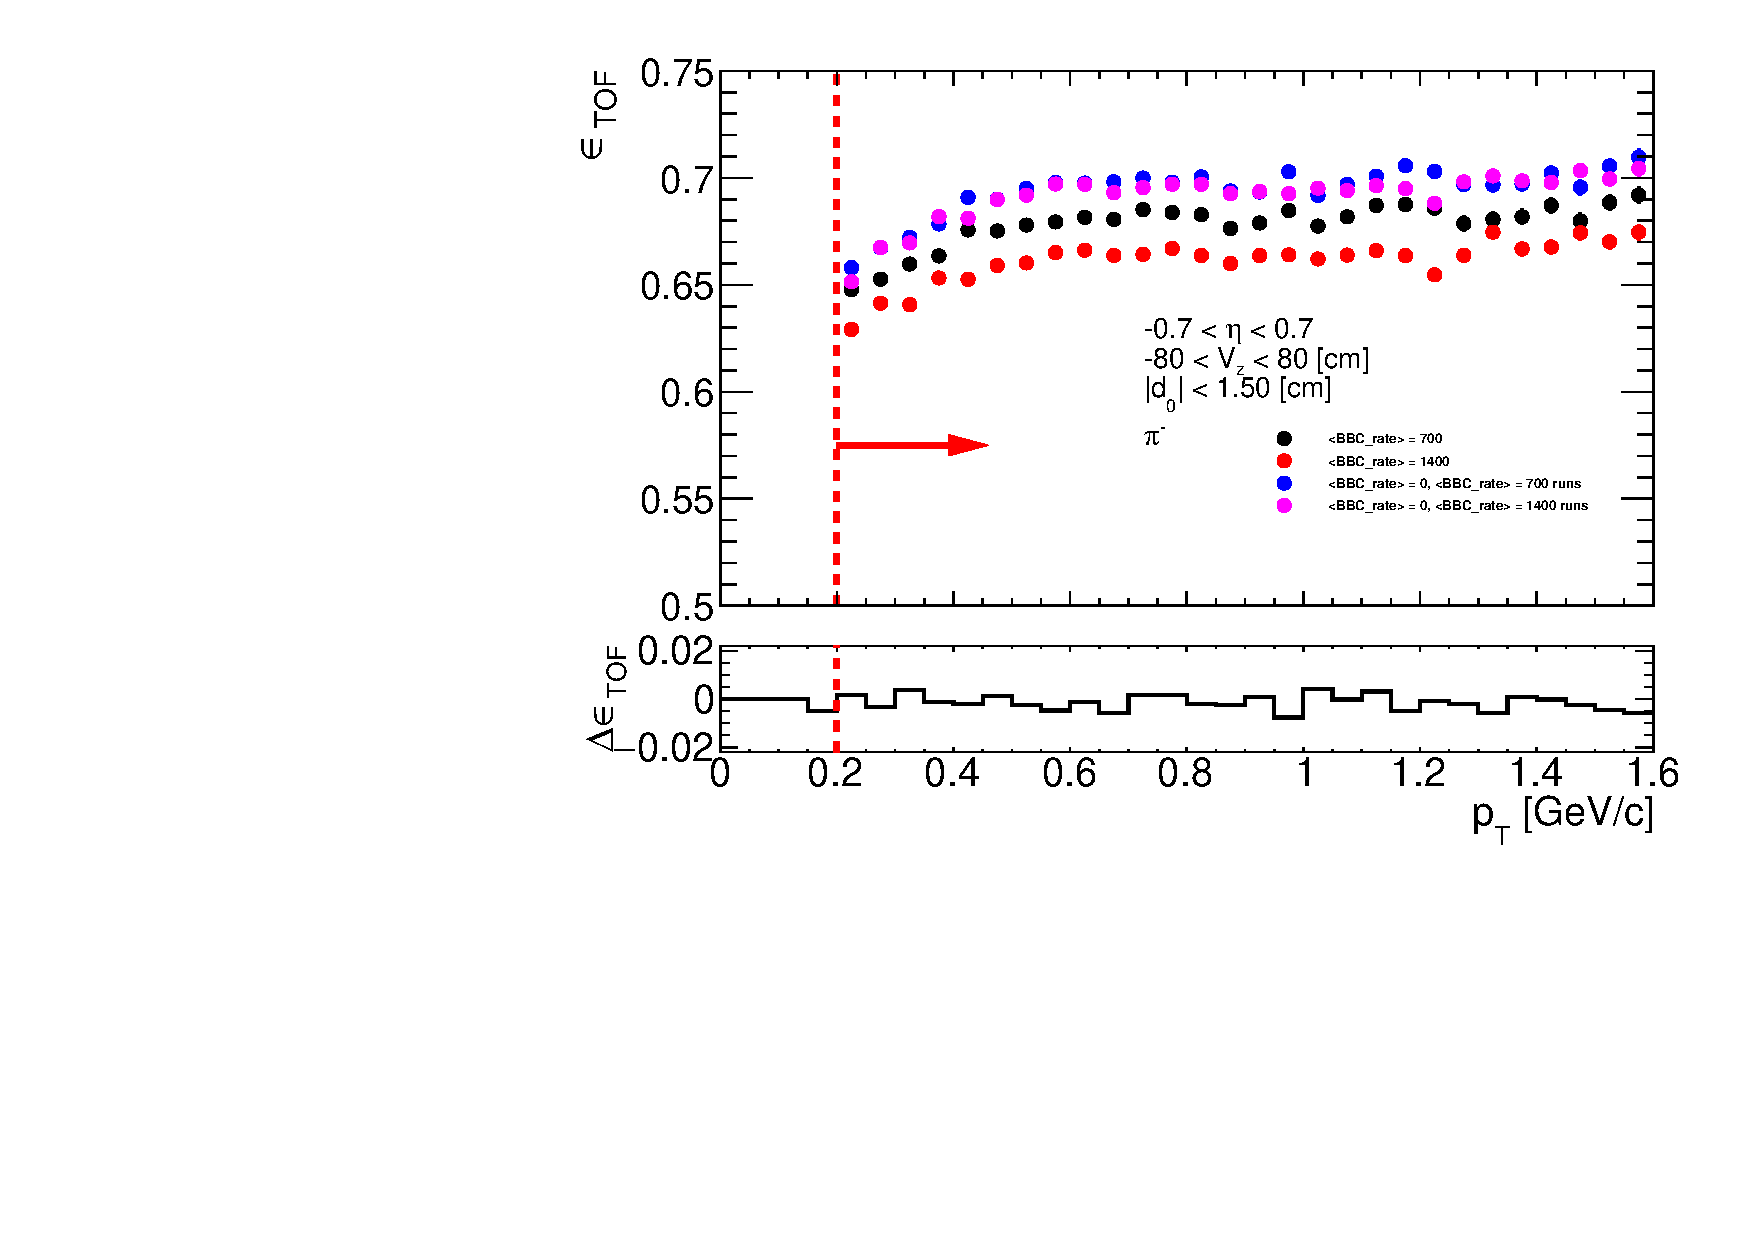
\includegraphics[width=\linewidth,page=1]{graphics/systematicsEfficiency/bbc_and/tofEffi_d0_1_5_etapt_1.pdf}\\
	}~
	\parbox{0.495\textwidth}{
		\centering
		\includegraphics[width=\linewidth,page=2]{graphics/systematicsEfficiency/bbc_and/tofEffi_d0_1_5_etapt_1.pdf}\\
	}%
\end{figure}
\begin{figure}[H]
	\caption[The difference $\Delta\epsilon_{ TOF} =\Delta\epsilon_{ TOF}^{1400\text{ kHz}}-2\cdot\Delta\epsilon_{ TOF}^{700\text{ kHz}}$ for $\pi^\pm$ as a function of $p_T$ and $\eta$ $\left(|V_z|<80\text{ cm}\right)$]{The difference $\Delta\epsilon_{ TOF} =\Delta\epsilon_{ TOF}^{1400\text{ kHz}}-2\cdot\Delta\epsilon_{ TOF}^{700\text{ kHz}}$ for $\pi^\pm$ as a function of $p_T$ and $\eta$ $\left(|V_z|<80\text{ cm}\right)$. }
	\label{fig:systError2Dtof}
	\centering
	\parbox{0.495\textwidth}{
		\centering
		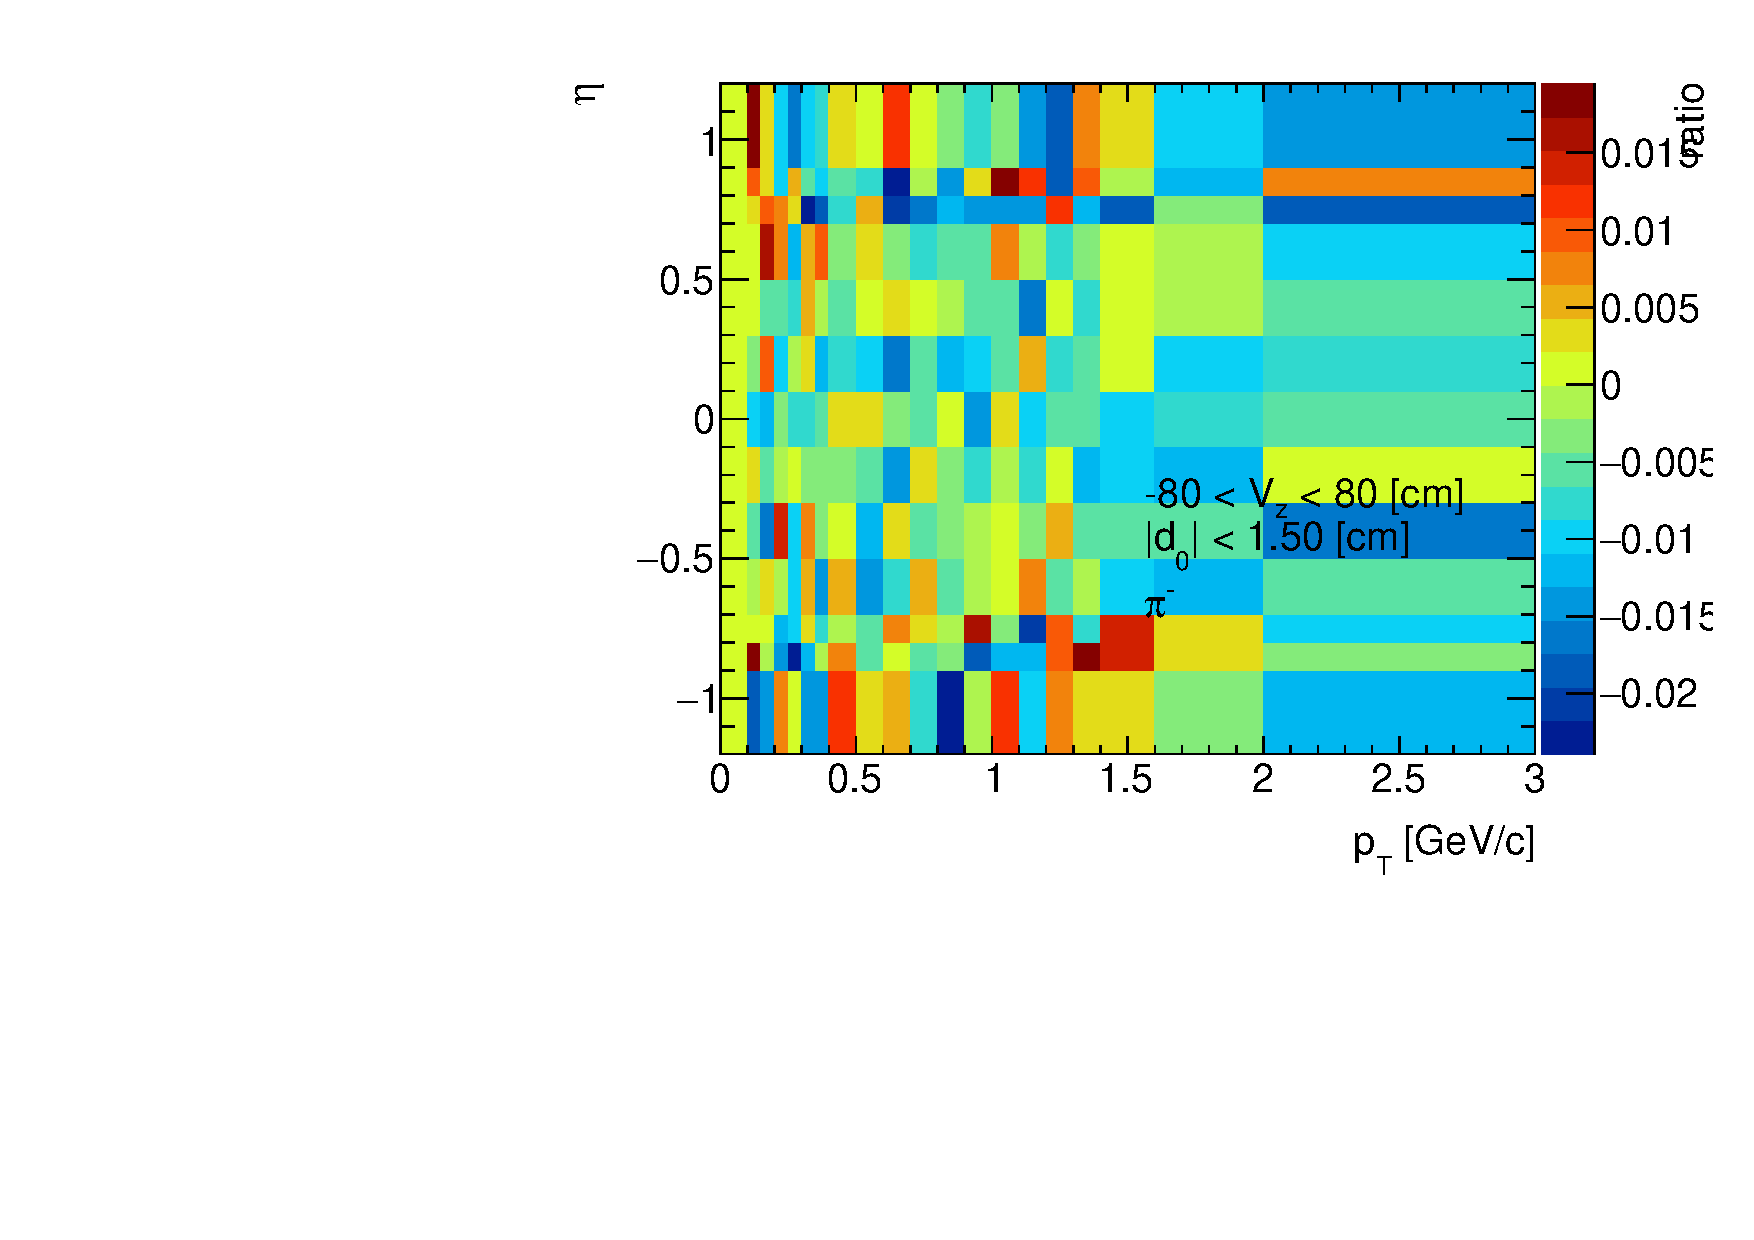
\includegraphics[width=\linewidth,page=1]{graphics/systematicsEfficiency/bbc_and/tofEffi_d0_1_5_etapt_12D.pdf}\\
	}~
	\parbox{0.495\textwidth}{
		\centering
		\includegraphics[width=\linewidth,page=2]{graphics/systematicsEfficiency/bbc_and/tofEffi_d0_1_5_etapt_12D.pdf}\\
	}%
\end{figure}



\subsection{Absolute error on TOF efficiency}\label{subsec:tofAbsEffSystAndCorr}

Systematic uncertainty of the TOF efficiency related to the accuracy of the TOF system simulation in STARsim and the TOF efficiency correction derived in Sec.~\ref{sec:tofAbsEffCorr} was estimated by comparing that nominal TOF efficiency with the one obtained with an independent method described below.

In some STAR analyses the TOF hit reconstrucion and matching efficiency is determined from the data with the use of BEMC: real (in-time) tracks are selected based on the fact that they match to BEMC cluster. If they do, the TOF efficiency is calculated as a ratio of number of TOF-matched tracks to number of all tracks. This solution may provide slightly biased efficiency, because the signal in the detector placed behind TOF, such as BEMC, ensures that particle followed the original helical path between the last hit of the track in TPC and the BEMC (Fig.~\ref{fig:hftEffSketch}).% Such efficiency may be higher than the efficiency without BEMC matching requirement.

We decided to calculate the TOF efficiency using the TPC tracks containing hits in HFT.... % The HFT is a silicon detector which 
%---------------------------
\begin{figure}[h]%\vspace{-2pt}%
\centering%
\begin{minipage}{.4725\textwidth}%
  \centering%\vspace{11pt}
  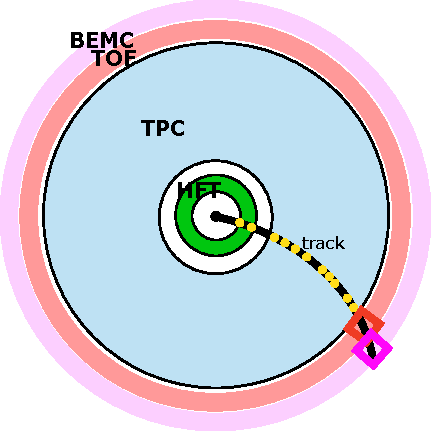
\includegraphics[width=0.965\linewidth]{graphics/systematicsEfficiency/TofSyst/effSketch.pdf}%\vspace{-5pt}%
  \caption[Sketch of the track with points in HFT.]%
  {Sketch of the cross section of the central detector and the track reconstructed with points in HFT. Presence of HFT points in a reconstructed track can be used as a tagger of the in-time tracks.}
  \label{fig:hftEffSketch}
\end{minipage}%
\quad\quad%
\begin{minipage}{.4725\textwidth}%
  \centering%
  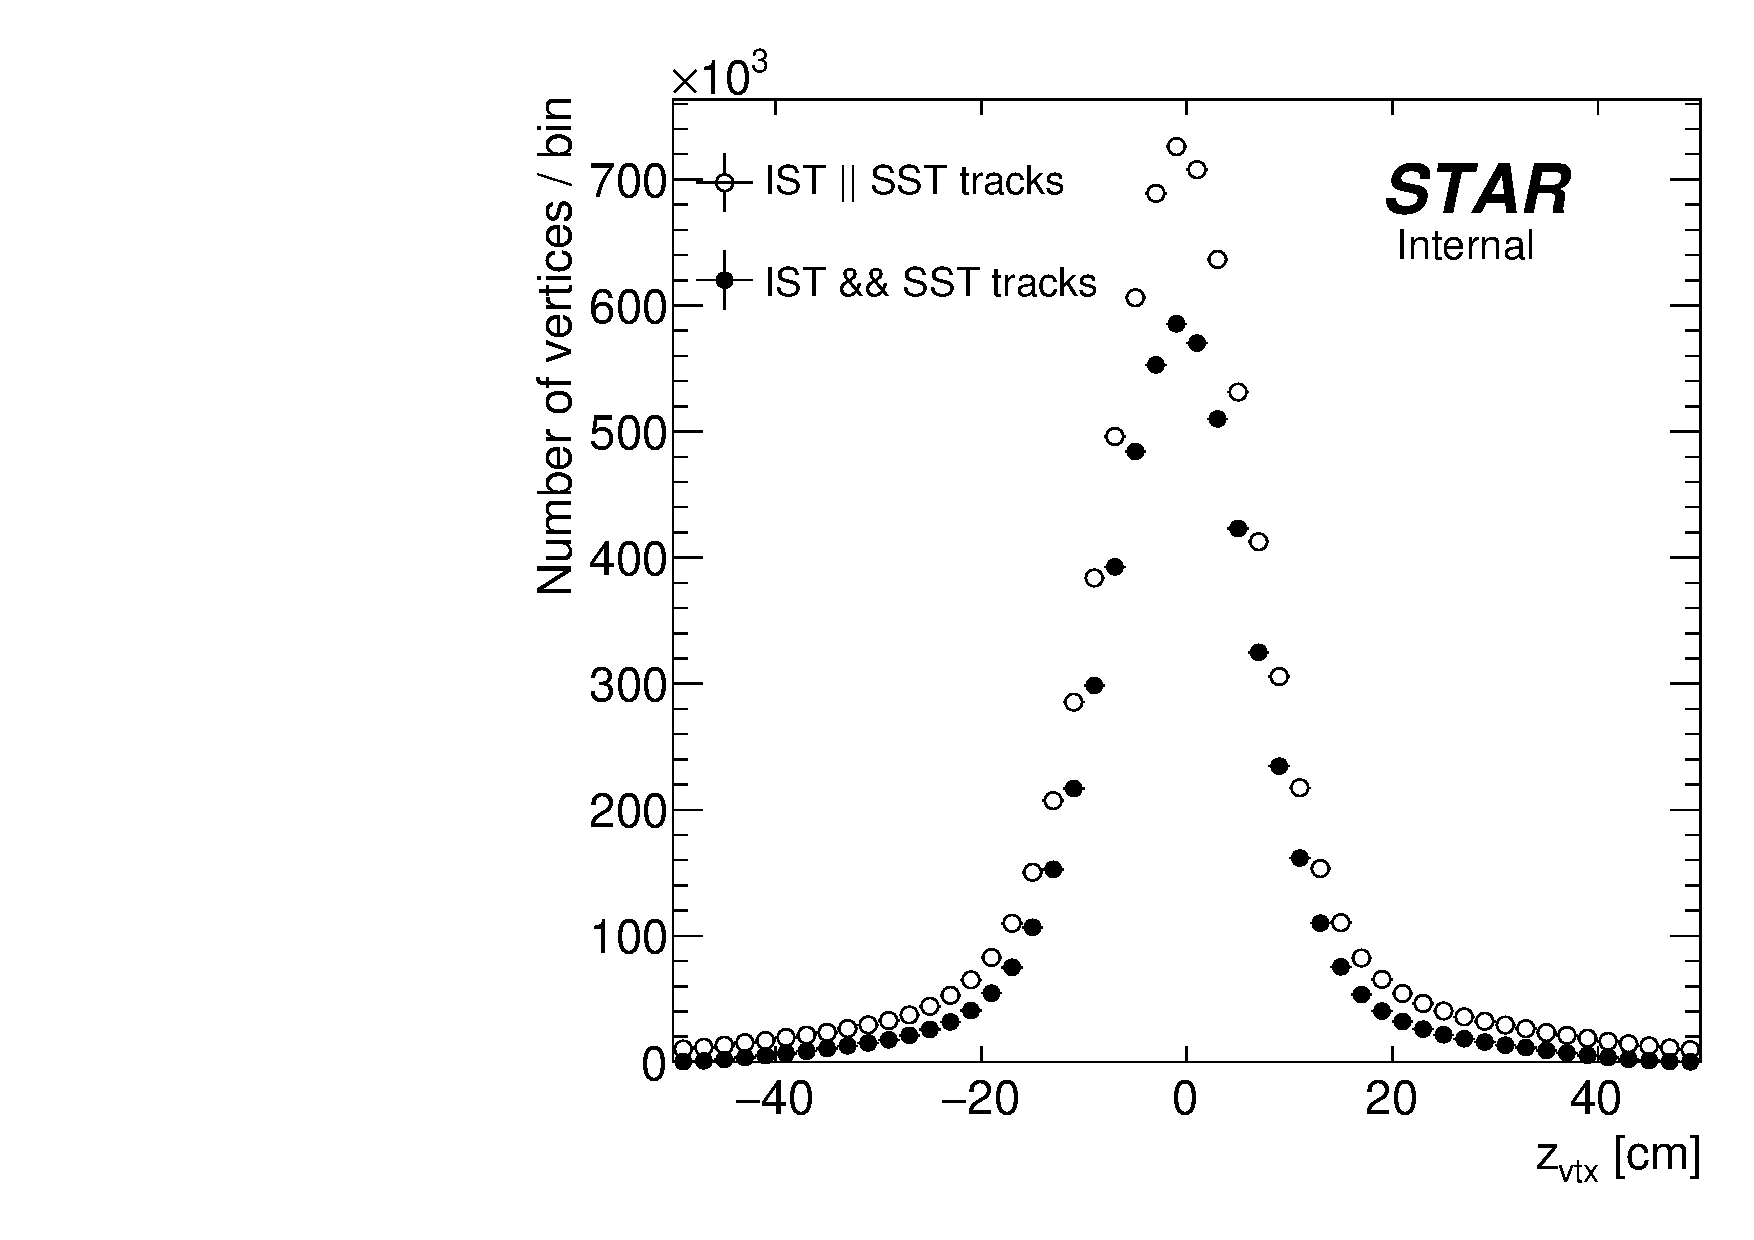
\includegraphics[width=\linewidth]{graphics/systematicsEfficiency/TofSyst/zVtxHFT.pdf}%\vspace*{-5pt}
  \caption[Distribution of $z$-position of vertices with TPC tracks containing hits in HFT.]
   {Distribution of $z$-position of vertices containing TPC tracks with HFT hits (st\_ssd stream). Open circles represent vertices with tracks with hits in IST or SST, full circles - IST and SST.}
   \label{fig:zVtxHFT}%\vspace*{-29pt}
\end{minipage}%
\end{figure}%
%---------------------------


%---------------------------
\begin{figure}[h!]
\centering
\parbox{0.31\textwidth}{
  \centering
  \begin{subfigure}[b]{\linewidth}{
                \subcaptionbox{\label{fig:aaa}}{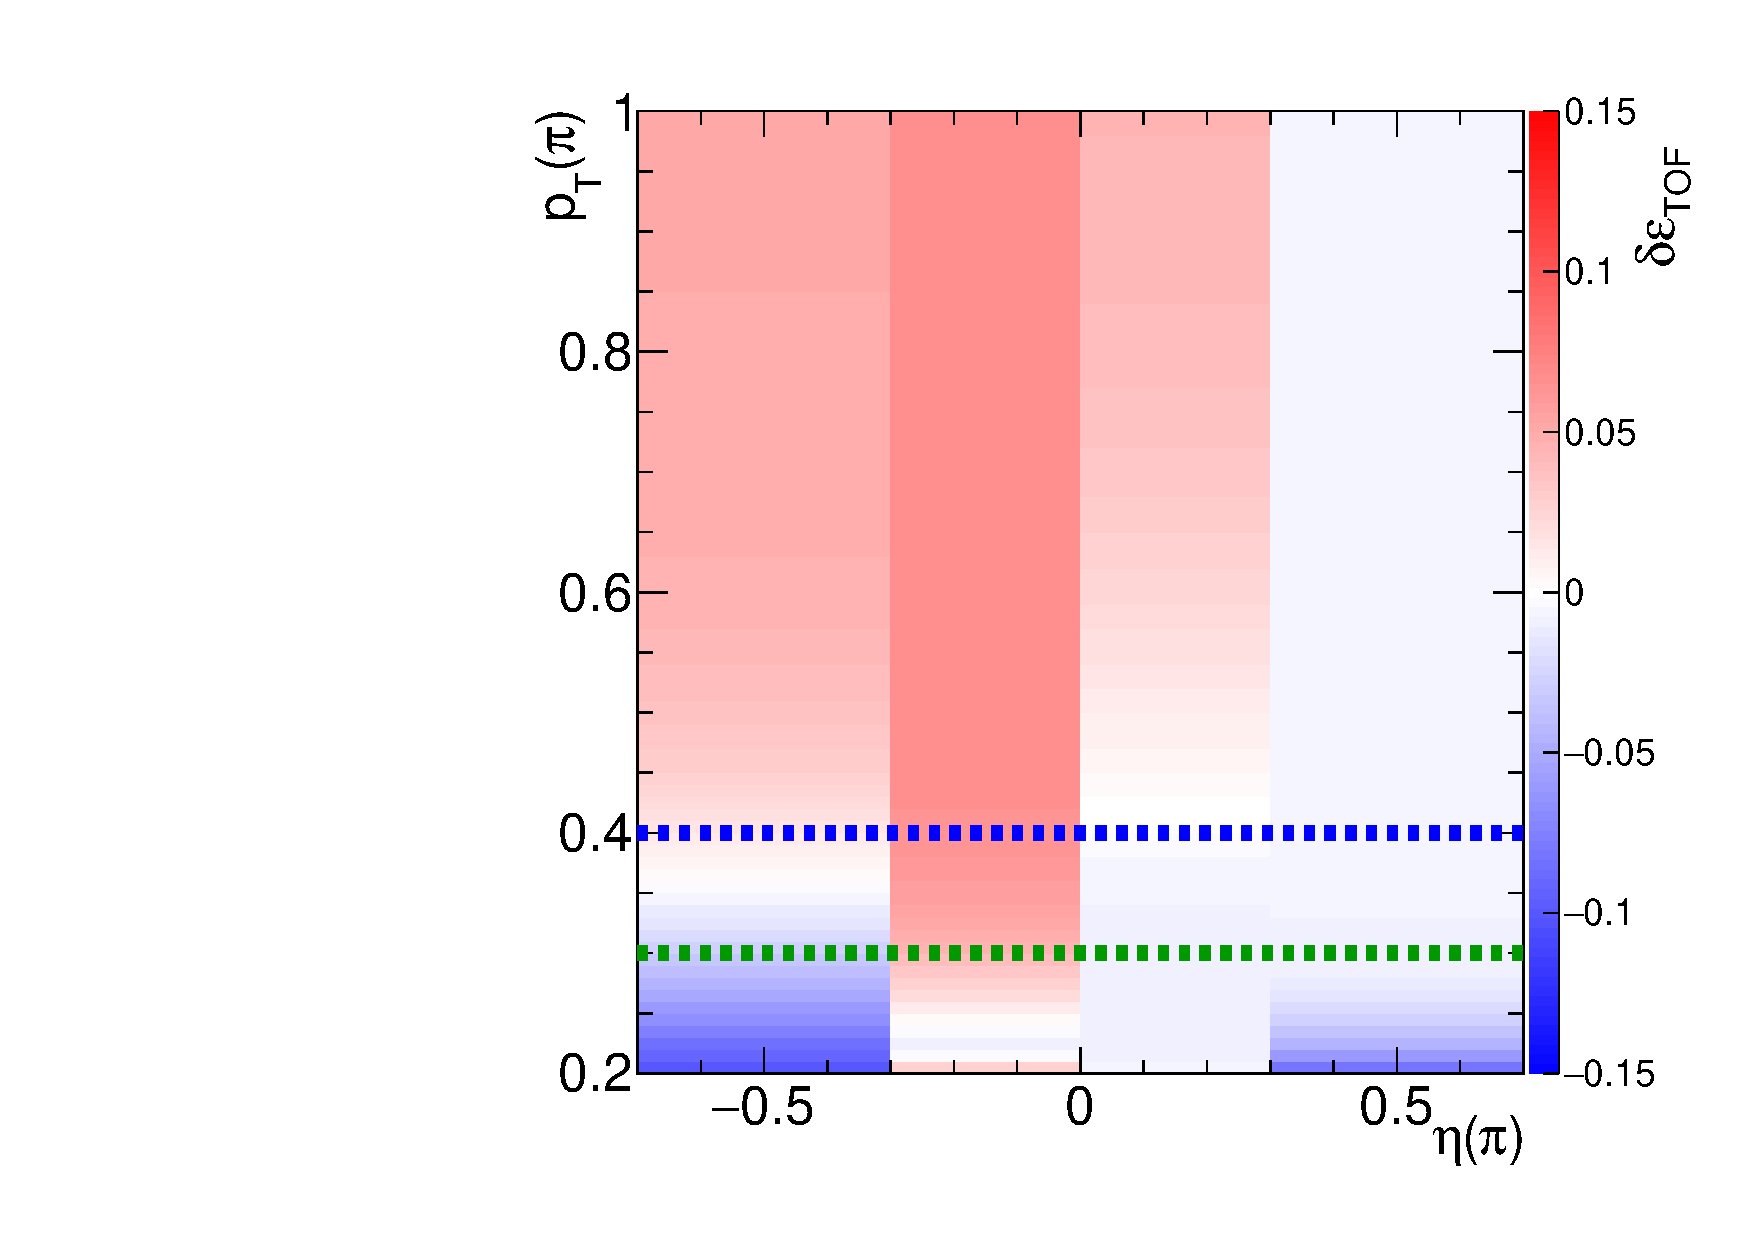
\includegraphics[width=\linewidth]{graphics/systematicsEfficiency/TofSyst//TofEffCorrection2D_pion.pdf}\vspace{-10pt}}}
  \end{subfigure}
}
\quad
\parbox{0.65\textwidth}{
  \centering
		\begin{minipage}[t][0.64\linewidth][t]{\linewidth}\vspace{30pt}
			\caption[Temporary.]%
    {Temporary.}\label{fig:erwetwet}%
		\end{minipage}
}\\[-20pt]
\parbox{0.31\textwidth}{
  \centering
  \begin{subfigure}[b]{\linewidth}{
                \subcaptionbox{\label{fig:aaa}}{\includegraphics[width=\linewidth,page=4]{graphics/systematicsEfficiency/TofSyst//tofEffDifference_pion.pdf}\vspace{-10pt}}}
  \end{subfigure}\\
  \begin{subfigure}[b]{\linewidth}\addtocounter{subfigure}{1}{
                \subcaptionbox{\label{fig:bbb}}{\includegraphics[width=\linewidth,page=5]{graphics/systematicsEfficiency/TofSyst//tofEffDifference_pion.pdf}\vspace{-10pt}}}
  \end{subfigure}\\
  \begin{subfigure}[b]{\linewidth}{
                \subcaptionbox{\label{fig:aaa}}{\includegraphics[width=\linewidth,page=6]{graphics/systematicsEfficiency/TofSyst//tofEffDifference_pion.pdf}\vspace{-10pt}}}
  \end{subfigure}\\
  \begin{subfigure}[b]{\linewidth}\addtocounter{subfigure}{1}{
                \subcaptionbox{\label{fig:bbb}}{\includegraphics[width=\linewidth,page=7]{graphics/systematicsEfficiency/TofSyst//tofEffDifference_pion.pdf}\vspace{-10pt}}}
  \end{subfigure}
}
\quad
\parbox{0.31\textwidth}{
  \centering
  \begin{subfigure}[b]{\linewidth}{
                \subcaptionbox{\label{fig:aaa}}{\includegraphics[width=\linewidth,page=3]{graphics/systematicsEfficiency/TofSyst//tofEffDifference_kaon.pdf}\vspace{-10pt}}}
  \end{subfigure}\\
  \begin{subfigure}[b]{\linewidth}\addtocounter{subfigure}{1}{
                \subcaptionbox{\label{fig:bbb}}{\includegraphics[width=\linewidth,page=4]{graphics/systematicsEfficiency/TofSyst//tofEffDifference_kaon.pdf}\vspace{-10pt}}}
  \end{subfigure}\\
  \begin{subfigure}[b]{\linewidth}{
                \subcaptionbox{\label{fig:aaa}}{\includegraphics[width=\linewidth,page=5]{graphics/systematicsEfficiency/TofSyst//tofEffDifference_kaon.pdf}\vspace{-10pt}}}
  \end{subfigure}\\
  \begin{subfigure}[b]{\linewidth}\addtocounter{subfigure}{1}{
                \subcaptionbox{\label{fig:bbb}}{\includegraphics[width=\linewidth,page=6]{graphics/systematicsEfficiency/TofSyst//tofEffDifference_kaon.pdf}\vspace{-10pt}}}
  \end{subfigure}
}
\quad
\parbox{0.31\textwidth}{
  \centering
  \begin{subfigure}[b]{\linewidth}{
                \subcaptionbox{\label{fig:aaa}}{\includegraphics[width=\linewidth,page=3]{graphics/systematicsEfficiency/TofSyst//tofEffDifference_proton.pdf}\vspace{-10pt}}}
  \end{subfigure}\\
  \begin{subfigure}[b]{\linewidth}\addtocounter{subfigure}{1}{
                \subcaptionbox{\label{fig:bbb}}{\includegraphics[width=\linewidth,page=4]{graphics/systematicsEfficiency/TofSyst//tofEffDifference_proton.pdf}\vspace{-10pt}}}
  \end{subfigure}\\
  \begin{subfigure}[b]{\linewidth}{
                \subcaptionbox{\label{fig:aaa}}{\includegraphics[width=\linewidth,page=5]{graphics/systematicsEfficiency/TofSyst//tofEffDifference_proton.pdf}\vspace{-10pt}}}
  \end{subfigure}\\
  \begin{subfigure}[b]{\linewidth}\addtocounter{subfigure}{1}{
                \subcaptionbox{\label{fig:bbb}}{\includegraphics[width=\linewidth,page=6]{graphics/systematicsEfficiency/TofSyst//tofEffDifference_proton.pdf}\vspace{-10pt}}}
  \end{subfigure}
}

\end{figure}
%---------------------------

